
\subsection*{Covariance estimation}
We aim to estimate the true covariance matrix 
\begin{equation}
\Sigma = \E{(x-\mu)(x-\mu)^\T}
\end{equation}
where $\E{\cdot}$ denotes expectation; $x$ is the $p\times 1$ vector of real-valued instantaneous firing rates in bins of duration $\Delta t$. The vector of mean firing rates is $\mu = \E{x}$.  

The usual estimator of the covariance matrix is the \emph{sample covariance matrix} computed from the empirical sample  $x(1),\ldots,x(n)$:
\begin{equation}
\hat \Sigma_0 = \frac 1 \nu \sum\limits_{t=1}^n (x(t)-\mu)(x(t)-\mu)^\T, 
\end{equation}
where $x(t)$ are sequential observations of population activity and $\nu$ is the number of degrees of freedom ($\nu=n-1$ if observations are independent).

The sample covariance matrix is unbiased i.e.\;$\E{\hat\Sigma_0}-\Sigma=0$.  For finite sample sizes, however, $\hat\Sigma_0$ is not as close to $\Sigma$ as a number of biased estimators that rely on \emph{regularization}. Regularization is the deliberate biasing of the estimate toward a low-dimensional, less variable \emph{target estimate} to strike a favorable balance between bias and variability of the estimate \cite{Bickel:2006,Ledoit:2004}.  

The estimator whose target estimate most closely matches the true low-dimensional structure of the data is likely to outperform other estimators. This principle provides the logic of this study. 

We considered four regularized estimators based on distinct families of low-dimensional target estimates: independent, latent factors, sparse partial correlations, and sparse partial correlations with latent factors. These target estimates are depicted graphically in Fig.~\ref{fig:03}A-D.  

The relative performance of the four estimators on synthetic and empirical data was evaluated by cross-validated multivariate normal log-likelihood (see Methods for detailed justification).  
Each estimator has one or two \emph{hyperparameters}, which are estimated within training datasets by nested cross-validation (See Methods). 

In the first regularized estimator, the target estimate is the diagonal matrix $\hat D$ containing on its diagonal estimates of the variances for each neuron.  The optimized estimate $\hat\Sigma_{\rm diag}$ is obtained by the linear \emph{shrinkage} of the unbiased estimate $\hat\Sigma_0$ toward $\hat D$ as regulated by scalar \emph{shrinkage intensity} $\lambda \in [0, 1]$:
\begin{equation}
\hat \Sigma_{\sf diag} = (1-\lambda) \hat \Sigma_0 + \lambda \hat D
\end{equation}
The diagonal target estimate expresses the idea of lack of dependence (or of linear association) between the activity of observed neurons (Fig.~\ref{fig:03}A).  If this assumption aptly describes recorded data, then strong shrinkage toward $\hat D$ will add little bias while strongly reducing the variability of the estimate. 

In the second regularized estimator, the target estimate is the factor model $\hat F = \hat L \hat L^\T + \hat \Psi$ with $d$ factors so that $\hat L$ is the $p\times d$ matrix of \emph{factor loadings} and the diagonal matrix $\hat \Psi$ contains the independent variances of each neuron.
Then the estimate is 
\begin{equation}
\hat \Sigma_{\sf factor} = (1-\lambda) \hat \Sigma_0 + \lambda \hat F,
\end{equation}
This estiamtor has two hyperparameters: the number of factors $d$ and shrinkage intensity $\lambda$. The target estimate $\hat F$ expresses the assumption that correlated fluctuations in population activity are driven by a small number of latent factors that affect many cells while direct interactions between cells are insignificant (Fig.~\ref{fig:03}B).   

The third estimator is based on the assumption that all correlations are the result of direct linear interactions between a fraction of observed cell pairs.  This assumption is enforced by reducing to zero the majority of pairwise \emph{partial correlations} in the recorded population. While usual correlations are calculated from the marginal distribution without conditioning on all the other neurons, the partial correlation expresses the pairwise correlation conditioned on the activity of all the other cells.  If cells only exert linear effects on each other and all neurons are visible, partial correlations express the direct interactions between neurons. Therefore, this estimator is biased toward the assumption that correlations arise due to interactions between a subset of pairs of recorded neurons (Fig.~\ref{fig:03}C). When the partial correlation between a pair of neurons is zero, then the corresponding element of the inverse of the covariance matrix (often referred to as the \emph{precision matrix} or \emph{concentration matrix}) must be zero as well. Then the estimator is 
\begin{equation}
\hat\Sigma_{\sf sparse} = \hat S^{-1}
\end{equation}
where $\hat S$ is a sparse matrix with a large fraction of zeros in its off-diagonal elements. The estimate has one hyperparameter to regulate the sparsity (fraction of off-diagonal zeros) in $\hat\Sigma$.


Finally, we consider a fourth estimator, which allows for both common latent factors interacting with all recorded neurons and sparse interactions between the recorded neurons (Fig.~\ref{fig:03}D). This estimator has the form
$\rho$.
\begin{equation}
\hat\Sigma_{\sf sparse+latent} = (\hat S - \hat L\hat L^\T)^{-1},
\end{equation}
where, as above, $\hat S$ is a sparse matrix and $\hat L$ is a $d\times p$ matrix of factor loadings. The estimator has two hyperparameters: the number of latent units $d$ and the sparsity of local interactions 
\subsection*{Simulation}

To verify our approach and to illustrate the performance of the four regularized estimators, we constructed five model populations with different covariance structures. Each population contained 50~neurons. 
The first four populations matched the low-dimensional structure of our four estimators: independent (Fig.~\ref{fig:03}A), latent factors (Fig.~\ref{fig:03}B), sparse partial correlations (Fig.~\ref{fig:03}C) and low-rank combined with sparse inverse (Fig.~\ref{fig:03}D).  
In addition, we considered a fifth population that had no low-dimensional structure (Fig.~\ref{fig:03}\,E).

\begin{figure}[htp]
\centering
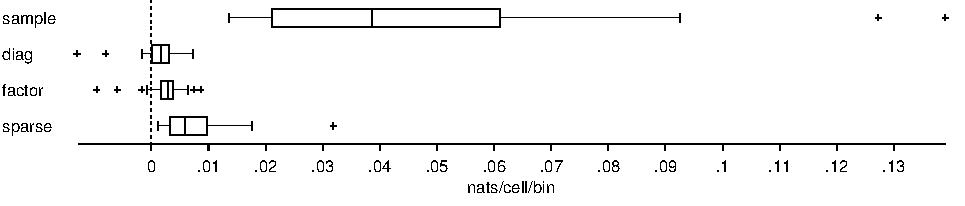
\includegraphics[width=1.0\textwidth]{figures/Figure3.pdf}
\caption{
Graphical models corresponding to the low-dimensional targets of the four regularization schemes used in the paper. It assumed that all interactions are linear, \emph{i.e.}\;the mean firing rate of any neuron can be computed by a linear combination of the firing rates of other neurons and latent units.
\textsf{A}: ``Independent.'' A population with no interactions corresponds to the diagonal covariance matrix.
\textsf{B}: ``Latent factors.'' Observed nodes are assumed to be influenced by several latent units (``factors") but are otherwise independent.
\textsf{C}: ``Sparse.'' Partial correlations between a subset of pairs of observed neurons, zero partial correlations between all other pairs.  
\textsf{D}: ``Sparse+latent.''  Partial correlations between a subset of pairs of observed neurons and a few latent factors interacting with the entire population. 
{\sf E--H} are examples of true $100\times100$ covariance matrices of multivariate normal distributions used in simulations. Matrix A has no low-dimensional structure. Matrices B--D have low-dimensional structture corresponding to the respective graphical models in Fig.~2B--D.
{\sf I--L} are examples of sample covariance matrices obtained from samples of size $n=1000$ from distributions with respective true covariance matrices A--D.
{\sf M--P:} Performance evaluation of covariance estimators A, B, C, D from samples obtained from models A, B, C, D.  Excess loss $\loss{\hat\Sigma,\Sigma}-\loss{\Sigma,\Sigma}$ is only accessible with the true covariance matrix $\Sigma$ is known and zero excess loss implies absolutely correct estimation. Estimators that can represent the graphical model outperform those that cannot.  Error bars indicate the standard deviation. 
{\sf Q--T:} Performance evaluation using \emph{validated loss} from Eq.~\ref{eq:validationLoss} without knowledge of true $\Sigma$. Cross-validation reproduces the same relationship between performances of the estimators.
}\label{fig:03}
\end{figure}

To evaluate the performance of the different estimators, we computed the excess loss for all combinations of model populations and estimators, including the sample covariance. The first striking observation is that in all cases all four regularized estimators performed substantially better than the sample covariance (Fig.~2, fourth row). In particular, this is even true for the case where the population did not have any low-dimensional structure at all (Fig.~2\,E). While it may appear surprising at first sight, this counter-intuitive phenomenon is known as \emph{Stein's phenomenon} or \emph{Stein's paradox} \cite{Efron:1977}, named after its discoverer Charles Stein \cite{Stein:1956}. A common misconception about regularization is that its effect depends on accurate prior knowledge about the structure of the data. However, substantial improvement can be attained by shrinking the unbiased estimate toward an arbitrary target as long as the target is less variable than the unbiased estimator. The more accurate description of regularization is as of the optimal tradeoff between estimation and approximation error -- the so-called ``bias-variance tradeoff''.

Thus, if taken in isolation a regularized estimator improves the estimate we should not interpret this result to suggest that the estimator's target has the same low-dimensional structure as the data-generating process. However, when comparing multiple estimators against each other, the one whose target estimate most closely matches the true value with the smallest number of parameters will reduce the estimation error with the least increase in approximation error. Indeed, in all four toy examples with a low-dimensional structure, the estimator with the matching regularization target performed best (Fig.~\ref{fig:03}\,A--D, fourth row). 
Since the estimator combining low-rank and sparse interactions combines to low-dimensional targets and includes the simpler estimators as special cases, it performed almost as well even when the low-dimensional structure did not include either a low-rank component or sparse interactions (Fig.~\ref{fig:03}\,B,\,C). 

Since the above evaluations of excess loss require knowledge of ground truth, this analysis can be done only on simulated data. However, \emph{validation loss} can be used as an unbiased empirical estimate of loss  (see Methods, Eq.~\ref{eq:validationLoss}. Validation loss uses an independent validation sample to estimate the value of loss without access to ground truth.   Indeed, this analysis revealed a pattern of results that reproduced the results obtained with access to ground truth above (Fig.~\ref{fig:03}, last row). Because validation loss is computed by comparing estimates to noisy sample covariance matrices from smaller validation sets, validation loss has higher variance than excess loss. Under our chosen loss function, validation loss does not converge to zero. 

\subsection*{Covariance estimation in neural data}


We recorded the calcium activity of dense populations of neurons in the supragranular layers in primary visual cortex of anesthetized mice using fast random-access 3D scanning two-photon microscopy \cite{Stosiek:2003,Reddy:2005}. We presented numerous repetitions of full-field drifting gratings (Fig.~\ref{fig:01}A and \ref{fig:01}B) to the eye contralateral to the imaged site. This technique allowed us to record from a large number (150--350) of cells in a small volume of cortical tissue ($200\times200\times100$ $\mu$m$^3$) in layers 2/3 and 4. We deconvolved somatic calcium signals using sparse nonnegative deconvolution \cite{Vogelstein:2010} (Fig.~\ref{fig:01}C and \ref{fig:01}D) and subtracted the average stimulus response to remove averaged linear effects of the stimulus. From this residual response we computed the sample noise covariance matrix (Fig.~\ref{fig:01}E).

\begin{figure}[htp]
\begin{center}
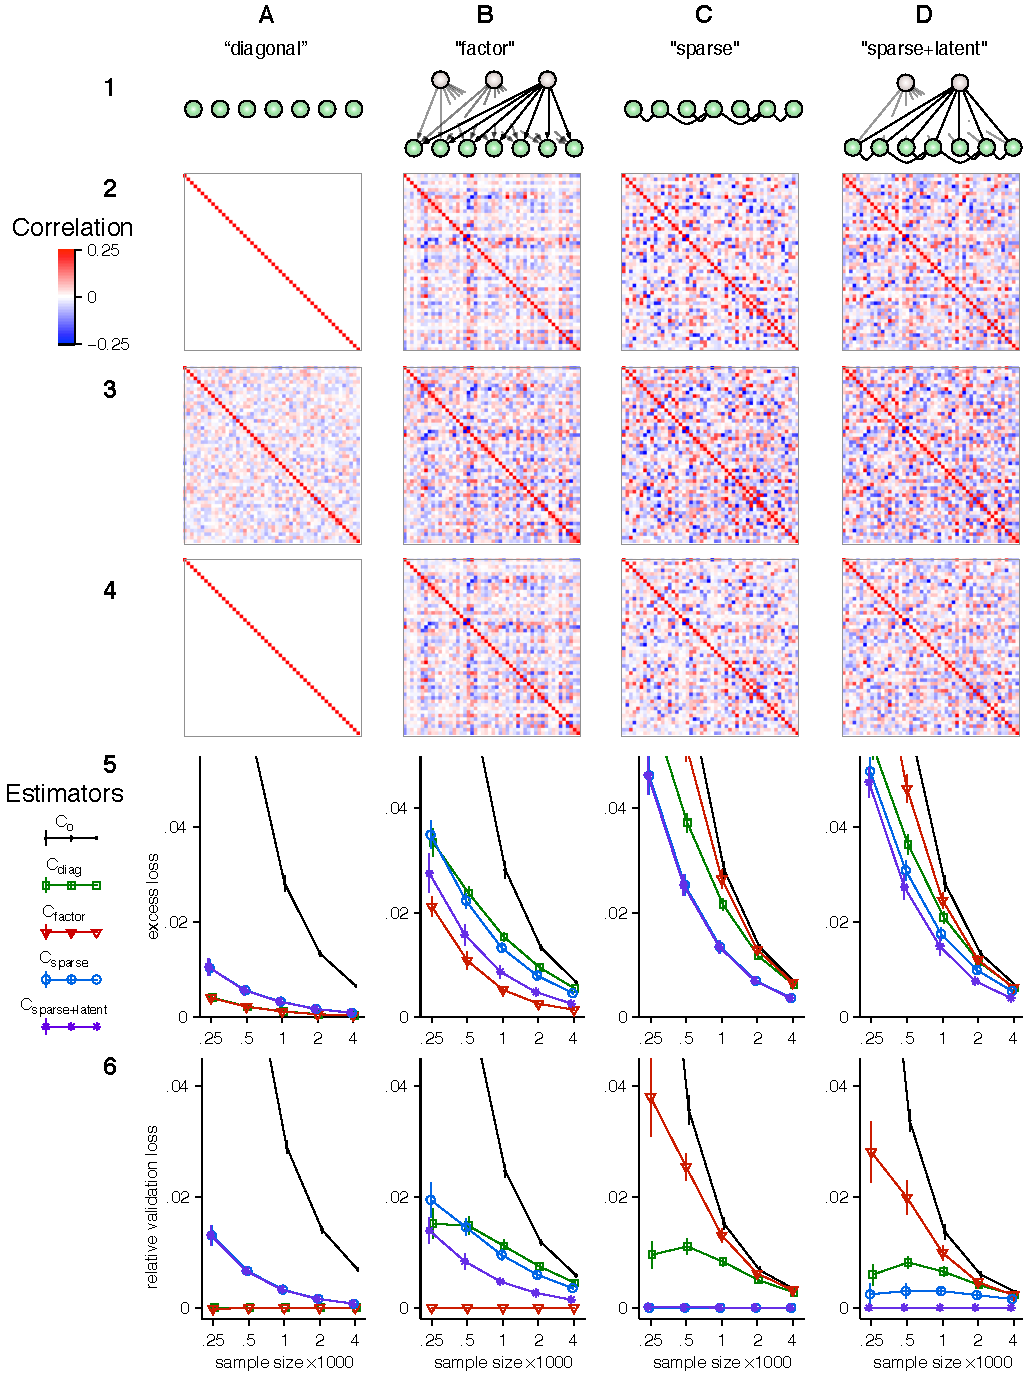
\includegraphics[width=2.5in]{figures/Figure1.pdf}
\end{center}
\caption{
{\bf Acquistion of neural population activity using two-photon fluorescence imaging of calcium signal.}  {\bf A.} Visual stimuli comprising brief (500 ms) presentatios of full-field drifting gratings separated by blank screens. {\bf B.} Two-photon fast 3D imaging of calcium signals in an awake mouse. {\bf C.} Deconvolved calcium signals. {\bf D.} The sample covariance matrix of neuronal calcium signals in 200 ms time bins. 
}
\label{Figure_label}
\end{figure}


In such highly localized populations both direct interactions between cells and common diffuse inputs are likely to contribute to the overall population variability. At the same time, most correlations are relatively small (Fig.~\ref{fig:01}E), suggesting that a simple shrinkage towards independence may provide a sufficiently well regularized estimate. By comparing the performance of our differently regularized estimators we can gain insights into which of these aspects are important in our data.

As expected, all regularized estimators outperformed the sample covariance estimator substantially (Fig.~\ref{fig:04}) \Acomment{I think we should show that}. Say something about how shrinkage, low-rank and sparse inverse relate \Acomment{Why do we do pairwise comparisons instead of just showing median (across sites) log loss relative to the combined estimator? I've seen many people do this and it provides an ordering. I feel like we should come up with a way of ordering them somehow, even if it's under certain assumptions that may not be entirely correct. I'm pretty sure if we don't do it the reviewers will bring it up anyway...}. Finally, the combined sparse and low-rank estimator dominated all others significantly (Fig.~4), showing that both hidden units and direct interactions are important in our data. The improvement from the low-rank estimator to the combined one is much larger than that from the sparse inverse to the combined one, suggesting that in this dataset direct interactions contribute more strongly to the correlation structure than hidden units do.

\begin{figure}[htp]
\centering
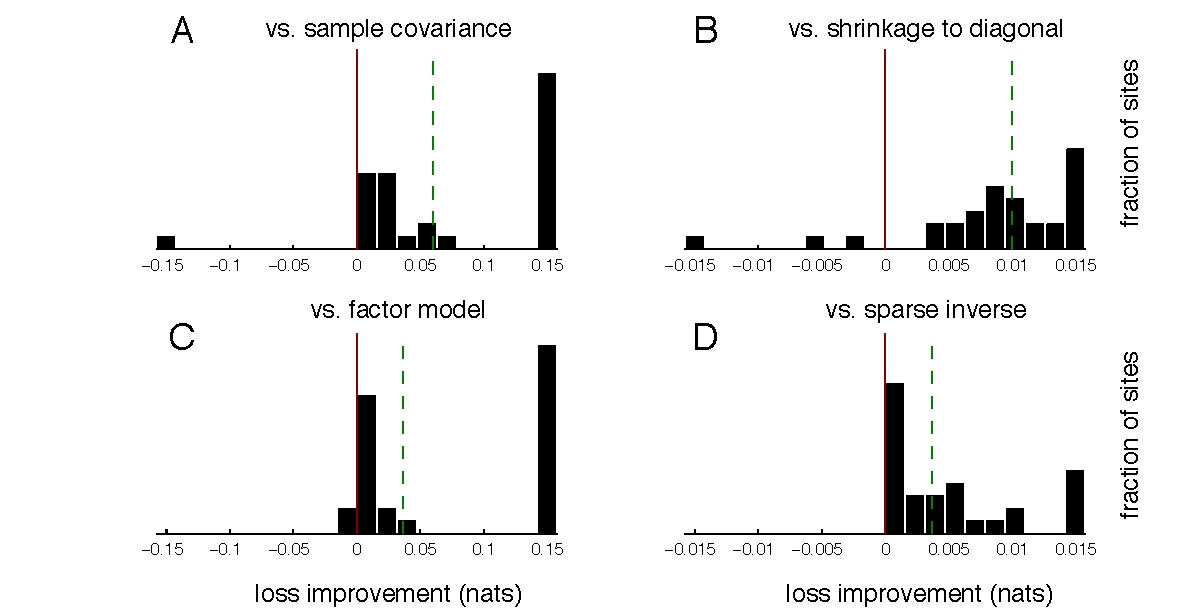
\includegraphics[width=0.5\textwidth]{figures/Figure4.pdf}
\caption{{\bf Estimator $\mathcal D$ (sparse+low-rank inverse covariance) dominates in dense recordings from primary visual cortex.}
{\bf A:}  Histogram of improvements in validation loss by covariance estimator $\mathcal D$ relative to the samle covariance matrix from the 31 imaged sites used in the study.  The vertical red line denotes the median improvment. 
{\bf B:} Improvements relative to estimator $\mathcal A$ (shrinkage toward the diagonal).
{\bf C:} Improvements relative to estimator $\mathcal B$ (shrinkage toward the factor model).
{\bf D:} Improvements relative to estimator $\mathcal C$ (sparse inverse covariance).
}\label{fig:04}
\end{figure}


\subsection*{Relationship between functional covariance structure and circuit architecture}
\begin{figure}[htp]
\centering
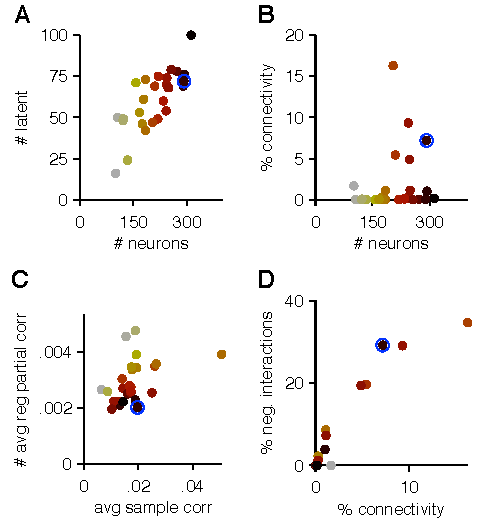
\includegraphics[width=0.5\textwidth]{figures/Figure5.pdf}
\caption{
Example of covariance structure revealed by the sparse+low-rank estimator and its relationship to the circuit arcitecture.
{\bf A:} The correlation matrix from Fig.~\ref{fig:01}D. 
{\bf B:} Optimal cross-validated sparse+low-rank estimate of the corrleation matrix from the same dataset. 
{\bf C:} Scaled negative inverse of the correlation matrix in {\bf A} (partial pairwise correlations). 
{\bf D:} Negative inverse of the sparse+low-rank estimate in {\bf B}. 
{\bf E:} The sparse component of {\bf D} with 96.5\% off-diagonal coefficients set to zero.
{\bf F:} The low-rank component of {\bf D}, rank=7.
{\bf G:} The spatial arrangement of cells used in the analysis, connected by edges that correspond to the non-zero elements of the sparse component in {\bf E}. Green edges denote positive weights, red edges denote negative weights.  Color-filled cells are significantly tuned to grating orientation as indicated by the color code in the legend.
}
\label{fig:05}
\end{figure}

\begin{figure}[htp]
\centering
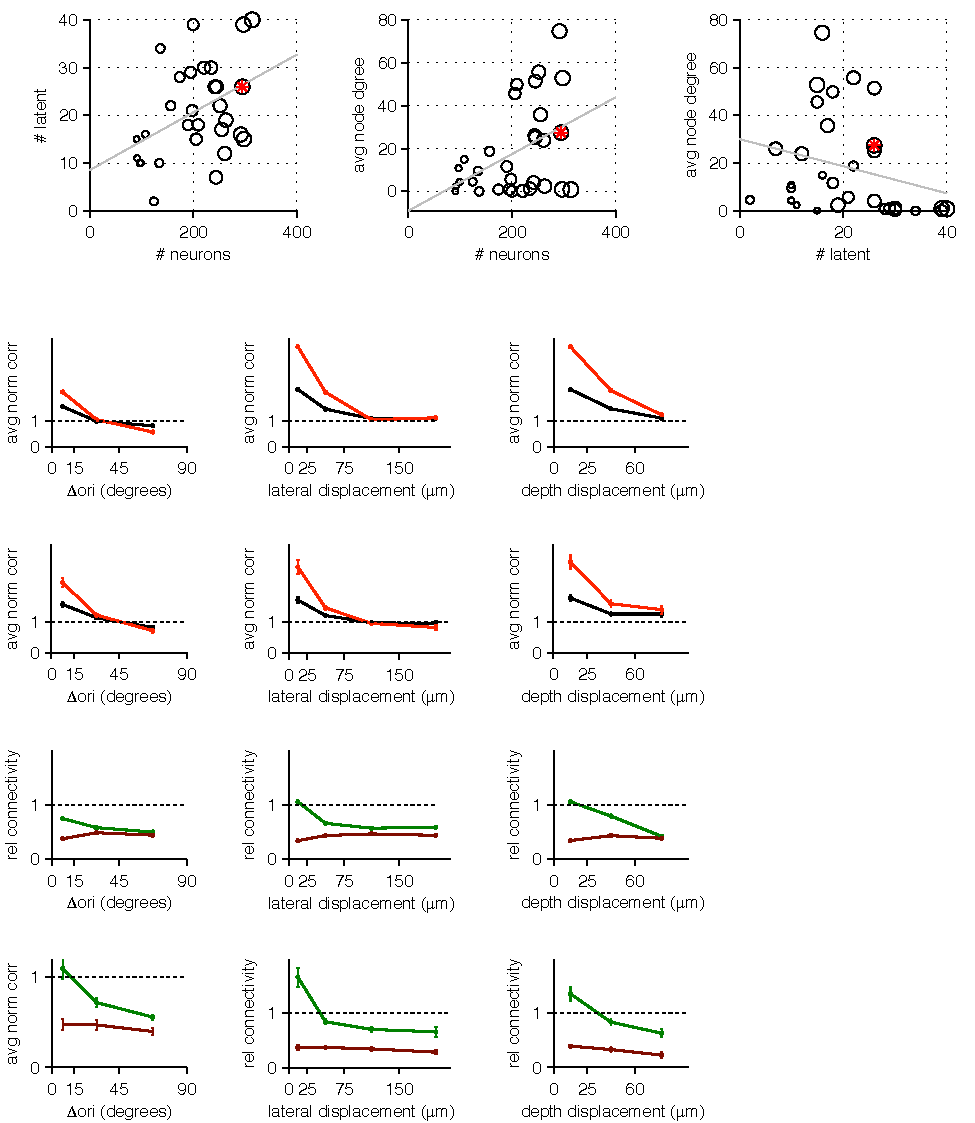
\includegraphics{figures/Summary.pdf}
\caption{
Relationship between the structure of the estimate and the functional and spatial organization of the circuit.
{\bf A:} Average sample correlation, average partial sample correlation, and average partial correlation in the sparse+low-rank estimate for site in Fig.~\ref{fig:05} as a function of difference in cortical depth within the same column.
{\bf C:} Average sample correlation, average partial sample correlation, and average partial correlation in the sparse+low-rank estimate for site in Fig.~\ref{fig:05} as a function of lateral distance at the same cortical depth.
{\bf E,G:} Average sample correlation, and interaction probability obtained from the sparse+low-rank estimate as well as by thresholding the sample correlation matrix to equal sparsity as function of difference in cortical depnth and lateral distance.
{\bf I:} Average sample correlation, and interaction probability obtained from the sparse+low-rank estimate as well as by thresholding the sample correlation matrix to equal sparsity as a function of difference in preffered orientation.
}
\label{fig:06}
\end{figure}


\begin{itemize}
\item Linear and partial correlations versus spatial separation (lateral and vertical). Discuss whether to include or remove thresholded correlations.
\item Magnitude of common input versus spatial location in the volume (lateral and vertical separation from center).
\item Linear and partial correlations versus orientation preference
\item Distribution of sparsity over sites
\item Distribution of number of hidden units over sites
\item Distribution of eigenvalues for sample covariance versus combined estimator
\item etc. etc. 

\end{itemize}





